

\section{Alternative parent selection}
 This section will discuss two alternative forms of parent selection: tournament selection and fitness proportionate selection. 
 
 \subsection{Fitness proportionate selection}
 The fitness proportionate selection method assigns to each individual a probability of selection that is directly proportional to its fitness value. This is summed up in formula \ref{eq:fitness_prop}. Because the fitness function is to be minimised, the fitness values are inverted prior to calculating the probabilities. 
 \begin{equation} \label{eq:fitness_prop}
 P(i) = \dfrac{\dfrac{1}{f_i}}{\sum\limits_{j=1}^\mu {\dfrac{1}{f_j}}}
 \end{equation}
 Next, Stochastic Universal Sampling (SUS) is used to select parents based on the probabilities obtained from \ref{eq:fitness_prop}.
 
 \begin{figure}[!]
\centering
\begin{subfigure}{0.45\textwidth}
  \centering
  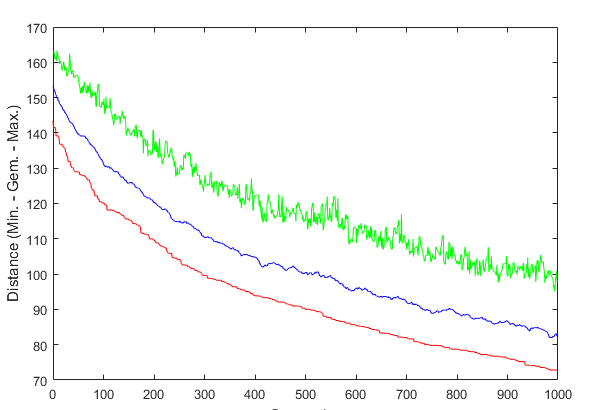
\includegraphics[width=1\textwidth]{../figures/question_5/FPS_off_gens.png}
      \caption{\textbf{Loop detection off} \textbf{Best tour distance found: $\mathbf{72.79}$, computation time: 390 seconds}. } 
      \label{fig:fps_vraag5_off_gen}
\end{subfigure}
\hspace{0.05\textwidth}
\begin{subfigure}{0.45\textwidth}
  \centering
  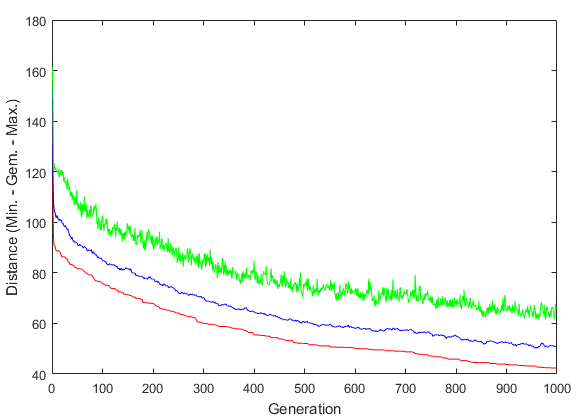
\includegraphics[width=1\textwidth]{../figures/question_5/FPS_on_gens.png}
      \caption{\textbf{Loop detection on)}.  \textbf{Best tour distance found: $\mathbf{42.1}$, computation time:357 seconds}.} 
      \label{fig:fps_vraag5_off_gen}
\end{subfigure}
\caption{The benchmark TSP problem \texttt{belgiumtour.tsp} with 380 cities is solved here using path representation with the following parameters: PR. MUT = $25\%$, PR. CROS = $60\%$ , ELITE = $5\%$. 200 individuals and 1000 generations.}
\label{fig:fps_gen}
\end{figure}

\begin{figure}{0.45\textwidth}[!]
\centering
 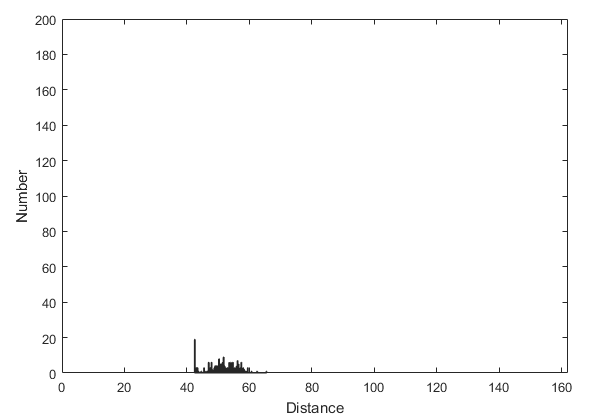
\includegraphics[width=1\textwidth]{../figures/question_5/FPS_hist.png}
 \caption{Histogram at 1000 generations using path representations with fitness proportionate selection.}
 \label{fig:fps_hist}
\end{figure}

